\documentclass[12pt]{article}
\usepackage[utf8]{inputenc}
\usepackage[T1]{fontenc}
\usepackage{amsmath}
\usepackage{graphicx}

\title{Response to the second report on the article draft \emph{The
    Impact of Gas Bulk Rotation on the Lyman-$\alpha$ line.}} 
\author{Juan N. Garavito-Camargo, Jaime E. Forero-Romero, Mark Disjkstra}
\date{\today}

\begin{document}


\maketitle

In what follows the comments by the referee are boldfaced.

Best regards, \\

The Authors\\


\section*{Global Comments}

\subsection*{Variations with viewing angle... again}

{\bf Figs 2 and 3 are very nice. They illustrate clearly the evolution
  of spectral shape with viewing angle. Note that the x label is
  wrong, it is not Vmax. It also needs a color bar to explicit the
  scale between a red pixel and a green/blue pixel. Because... to my
  eyes, there is an obvious third result illustrated on these Figs,
  which is that much less photons seem to escape at the equator than
  along the poles: the red pixels are concentrated towards the pole,
  whereas there seems to be less light emerging from equatorial
  directions. But if the dynamical range between red and blue is very
  small, maybe it’s ok, given that the equatorial spectrum is
  broader}

We have correctd the xlabel. Indeed the
concentration of photons in a narrow range of velocities along the
poles (i.e. red values) is compensated by a broader distribution
around the equator. The total number of photons is the same regardless
of the $\cos\theta$ value. This is the result of the test shown in
Figure 5. 




{\bf How did you select photons when you did this Fig 2 ? Did you
  select them on $|\cos\theta|$? You should select only one side, one
  hemisphere, otherwise you count twice more photons anywhere else
  than along the equator. Did you select a peculiar $\varphi$ ? Or did
  you sum over the azimuthal direction ? In order to avoid this
  impression that less photons escape at equator, you should indeed
  sum over $\varphi$. }

The 2D distribution is symmetric on $\cos\theta$. We mention this in
the first paragraph of the results section. Using this symmetry we select
by $|\cos\theta|$ in order to have less noise in the 2D histograms. We
also sum over $\varphi$.


{\bf However, these selection biases would also affect the static case, whereas the first column looks ok to me, it seems that the same “intensity” is escaping from all directions for this column, and not for the others.
It is in strong contradiction with your Fig 5. How do you explain this ?
Furthermore, I would have expected the contrary, with more photons escaping at the equator, where the velocity field is stronger, than through the poles, where everything is static... However, Ly$\alpha$ radiation transfer effects can often be far from intuitiv.}

The colors in the Figures 2 and 3 correspond to number densities
inside a velocity-$|\cos\theta|$ pixel. The total flux is thus an
integrated quantity over the velocity and should not be estimated from
the pixel intensity. It is difficult to visualize
the result from Figures 2 and 3. That's why we prepare Figure 5 to
show that the integrated flux is independent of the angle. 


\subsection*{intrinsic spectrum on Fig 4}

{\bf From your Figs 6 and 7, it seems that the results for central and homogeneous cases are very comparable. I would like to see the shape and FWHM of the intrinsic spectra (I mean before transfer) in the case of homogeneous sources, for the static case, as the fiducial case, and when Vmax=100,200,300 km/s, along the equatorial direction. I would like to infer how much of the broadening of the line is really due to transfer effects. Could you make a figure where you compare the intrinsic and emerging spectra along
the equatorial plane ?} 


The Figure is here:\\


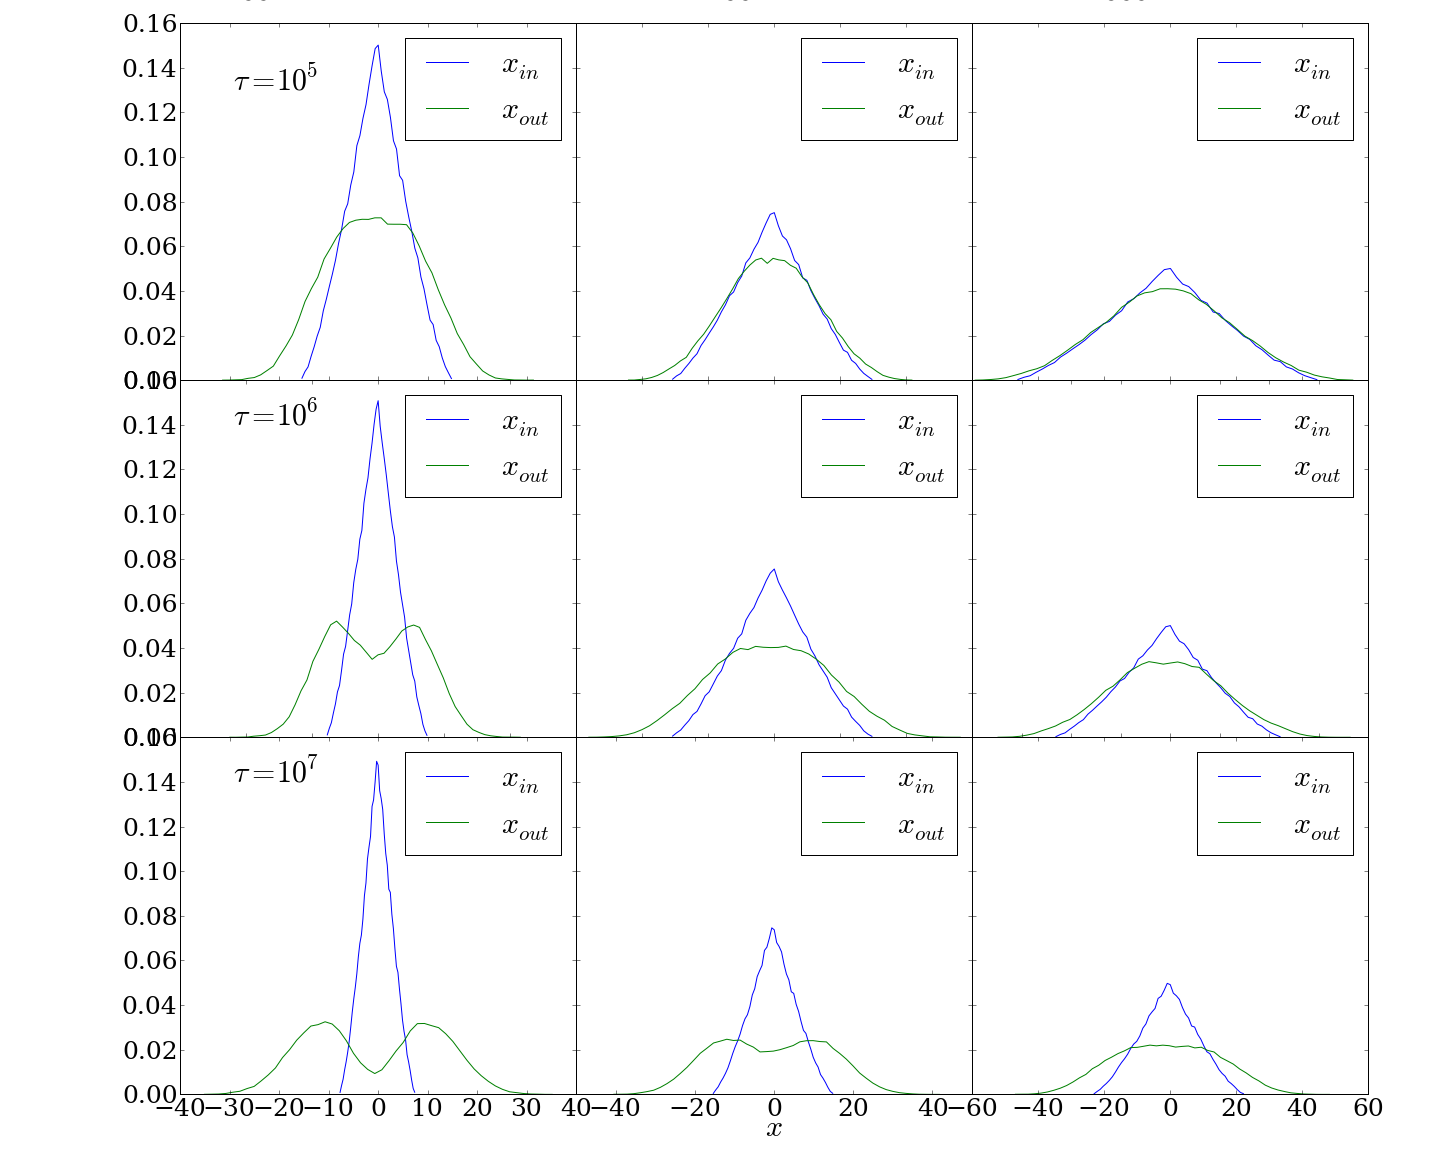
\includegraphics[width=1.0\textwidth]{../code/intrinsic_spectrum.png}


\subsection*{Sect 4.1 : Rotation = Static ?}

{\bf I don’t understand the reasonning that rotation would act on the Ly$\alpha$ transfer as a static medium, since Ly$\alpha$ photons are “co-rotating”. You mention this argument once in the “answer to referee” document, and once in the text Sect. 4.1, with a sentence which reads absurd : a rotating sphere is identical from a static one. At least, it is not well formulated.
It seems to me that your argument should be right for any kind of motion. Why would it be specific to rotation ? In other words, you could exchange the word “rotation” with the word “outflow” or “inflow” in your reasonning, right ? “While scattering events off atoms within the outflowing cloud impart Doppler boosts on the Ly$\alpha$ photon, these Doppler boost are only there in the lab-frame. Therefore, in the frame of the outflowing gas cloud all atoms are stationnary with respect to each other and the scattering process proceeds identical as in the static case.”. However, all atoms in a rotating/outflowing/infalling cloud are not stationary with respect to each other, otherwise the cloud would be static! Your reasonning is true at the scale of each cell, but not at global scale.
I did not understand the alternative -more quantitative- explanation better.
Can you develop this point ? Maybe, to convince me, you could look at the redistribution of frequencies after one single diffusion ( 1/ in all directions, 2/ along the rotation axis, 3/ in the equator plane), emitting your photons at a radius r = 0.9 R, and comapre them with the same redistributions in the static case. If they are identical, you are right, rotation does not have any effect... if they are different, multiple scatterings will have a cumulative effect on the spectral shape, but also on the probalility to escape more easily in some directions than others... I understand that this implies new simulations and more time, but I would really appreciate to see these plots. } 

\subsection*{Angular variation of the distribution of escaping directions}

{\bf It seems to me that Ly$\alpha$ photons escape a medium through the path of minimum optical depth. So, in a rotating cloud, where the velocity field is tangential, they might “rotate” or spiral from the center to the edge. To test this idea, you could look at the distribution of escaping directions from photons emerging at the pole or at the equator. But for this, you need to keep track of the location of escape, and not only of the direction of escape. Did you collect this information ?
I would expect that photons at the equator escape more tangentially to the sphere than at the poles... But again, Ly$\alpha$ transfer is not exactly intuitiv.}


\section*{Details}

\subsection*{Sect. 3.1}

{\bf You say that “If the viewing angle is aligned with the rotation axis, $|\mu| \approx 1$, the Ly$\alpha$ line keeps in most of the cases a double peak”, isn’t it in all cases ?}

\subsection*{Sect. 3.5}
{\bf The parameter a is not defined when you discuss Neufeld.} 

\subsection*{Fig9}

{\bf Is Fig 9, left panel, for a central source ? Can you show the homogeneous case also ? You discuss in the referee repport that the distribution is not bimodal anymore. But it has to be different than in central case, spanning the whole range of nb scatt, because photons are emitted at every radii in the cloud, so at every optical depth.
On the right panel, solid and dashed lines are not defined.} 

\subsection*{Vmax = 1000 km/s}
{\bf If you did this test and checked that the nb of scatterings and the escape fraction is still angle invariant for such a high velocity, then it is worth mentionning it. Because in principle, media with very high velocities should start to become transparent for Ly$\alpha$.} 

\end{document}
